% Supplementary material generated during COMST pass 1.
% These blocks were copied verbatim from the active manuscript before compression.
% They are not input by bare_jrnl_new_sample4.tex in this working pass.

% ---- Moved block: tab:performance_comparison ----
\begin{table*}[!t]
    \caption{RF-ISAC vs. O-ISAC Performance Comparison \protect\cite{O_ISAC_021}}
    \label{tab:performance_comparison}
    \centering
    \footnotesize
    \setlength{\tabcolsep}{3.2pt}
    \renewcommand{\arraystretch}{1.15}

    \begin{tabularx}{\textwidth}{@{}%
        >{\raggedright\arraybackslash}p{2.35cm}
        >{\raggedright\arraybackslash}X
        >{\raggedright\arraybackslash}X
        >{\raggedright\arraybackslash}X
        @{}}
        \toprule
        \textbf{Characteristic}                           &
        \textbf{RF-ISAC (Sub-6 GHz / mmWave)}             &
        \textbf{Wireless O-ISAC (FSO / VLC / Photo-THz)}  &
        \textbf{Wired O-ISAC (Fiber Sensing)}               \\
        \midrule

        \textbf{Carrier Frequency}                        &
        2.4--100 GHz                                      &
        0.1--10 THz (Photo-THz) + 28.3--845 THz (FSO/VLC) &
        193 THz (C-band / L-band)                           \\

        \textbf{Physics Model}                            &
        Diffuse multipath (rich)                          &
        LoS-dominated propagation                         &
        Guided mode (low-loss, dispersive)                  \\

        \textbf{Signal Type}                              &
        Complex (I/Q)                                     &
        Real (IM/DD) or complex (coherent FSO)            &
        Complex (coherent phase/polarization)               \\

        \textbf{Key Impairments}                          &
        Interference, multipath fading                    &
        Ambient light, turbulence, pointing error         &
        Kerr nonlinearity, PMD, phase noise                 \\

        \textbf{Sensing Task}                             &
        Radar (range/Doppler)                             &
        Localization, gesture, surface profiling          &
        DAS (vibration), strain, temperature                \\

        \textbf{Peak Data Rate}                           &
        $\sim$10--20 Gbps                                 &
        \textbf{$\sim$100--120 Gbps} \cite{O_ISAC_105}    &
        \textbf{$>$200 Tbps} (aggregate) \cite{O_ISAC_046}  \\

        \textbf{Resolution}                               &
        cm-level                                          &
        \textbf{mm-level (2.5 mm)} \cite{O_ISAC_105}      &
        m-level (spatial) / $n\varepsilon$ (strain)         \\
        \bottomrule
    \end{tabularx}

    \vspace{2pt}
    \footnotesize
    \emph{Abbreviations:} RF = radio frequency; FSO = free-space optics; VLC = visible light communication;
    Photo-THz denotes photonic-THz or optical--THz bridging links; DAS = distributed acoustic sensing;
    IM/DD = intensity modulation/direct detection; PMD = polarization mode dispersion.
\end{table*}

% ---- Moved block: tab:math_notation ----
\begin{table}[!t]
    \caption{Mathematical Notation Conventions}
    \label{tab:math_notation}
    \centering
    \footnotesize
    \begin{tabularx}{\columnwidth}{@{}>{\raggedright\arraybackslash}p{0.33\columnwidth} >{\raggedright\arraybackslash}X@{}}
        \toprule
        \textbf{Symbol}                                & \textbf{Definition}                                          \\
        \midrule
        $\lambda$                                      & Optical wavelength (nm)                                      \\
        $B_{\mathrm{eff}}$                             & Effective signal bandwidth (Hz)                              \\
        $R$                                            & Data rate (bit/s)                                            \\
        $d$                                            & Target distance or range (m)                                 \\
        $\Delta r_{\min}$                              & Bandwidth-limited two-way range resolution (m)               \\
        $\sigma_r = \sqrt{\mathbb{E}[(\hat r - r)^2]}$ & Range estimation error or RMSE (m)                           \\
        $\mathrm{SNR}$                                 & Signal-to-noise ratio                                        \\
        $\mathrm{BER}$                                 & Bit error rate                                               \\
        $\alpha$                                       & Power allocation factor for communication--sensing trade-off \\
        \bottomrule
    \end{tabularx}
\end{table}

% ---- Moved block: tab:acronyms ----
\begin{table}[!t]
    \caption{List of Frequently Used Acronyms}
    \label{tab:acronyms}
    \centering
    \footnotesize
    \begin{tabularx}{\columnwidth}{@{}>{\raggedright\arraybackslash}p{0.33\columnwidth}>{\raggedright\arraybackslash}X@{}}
        \toprule
        \textbf{Acronym}     & \textbf{Definition}                                                \\
        \midrule
        \textbf{ISAC}        & Integrated Sensing and Communication                               \\
        \textbf{O-ISAC}      & Optical Integrated Sensing and Communication                       \\
        \textbf{ISAC-OF}     & Integrated Sensing and Communication in Optical Fiber              \\
        \textbf{DFS}         & Distributed Fiber Sensing                                          \\
        \textbf{DAS}         & Distributed Acoustic Sensing                                       \\
        \textbf{VLC}         & Visible Light Communication                                        \\
        \textbf{FSO}         & Free-Space Optical                                                 \\
        \textbf{OWC}         & Optical Wireless Communication                                     \\
        \textbf{LFM}         & Linear Frequency Modulation                                        \\
        \textbf{OFDM}        & Orthogonal Frequency Division Multiplexing                         \\
        \textbf{DCO-OFDM}    & DC-biased Optical OFDM                                             \\
        \textbf{OCDM}        & Orthogonal Chirp Division Multiplexing                             \\
        \textbf{IM/DD}       & Intensity Modulation / Direct Detection                            \\
        \textbf{ORIS}        & Optical Reconfigurable Intelligent Surface                         \\
        \textbf{OPA}         & Optical Phased Array                                               \\
        \textbf{PIC}         & Photonic Integrated Circuit                                        \\
        \textbf{CCR}         & Corner Cube Reflector                                              \\
        \textbf{RO-ISAC}     & Retroreflective O-ISAC                                             \\
        \textbf{$\phi$-OTDR} & Phase-Sensitive Optical Time-Domain Reflectometry                  \\
        \textbf{SMF}         & Single-Mode Fiber                                                  \\
        \textbf{FMF}         & Few-Mode Fiber                                                     \\
        \textbf{MCF}         & Multi-Core Fiber                                                   \\
        \textbf{WDM}         & Wavelength Division Multiplexing                                   \\
        \textbf{DSCM}        & Digital Subcarrier Multiplexing                                    \\
        \textbf{THz}         & Terahertz                                                          \\
        \textbf{MIMO}        & Multiple-Input Multiple-Output                                     \\
        \textbf{PRISMA}      & Preferred Reporting Items for Systematic Reviews and Meta-Analysis \\
        \textbf{TQAF}        & Technical Quality Assessment Form                                  \\
        \textbf{RMSE}        & Root Mean Square Error                                             \\
        \textbf{CRB}         & Cram\'er--Rao Bound                                                \\
        \bottomrule
    \end{tabularx}
\end{table}

% ---- Moved block: tab:section6_notation ----
\begin{table}[!t]
    \caption{Unified Notation for Section VI}
    \label{tab:section6_notation}
    \centering
    \footnotesize
    \begin{tabularx}{\columnwidth}{@{}>{\raggedright\arraybackslash}p{1.85cm}>{\raggedright\arraybackslash}X>{\raggedright\arraybackslash}p{1.55cm}@{}}
        \toprule
        \textbf{Symbol}      & \textbf{Meaning}                                                                                             & \textbf{Used in}       \\
        \midrule
        $x(t)$               & Optical transmit waveform or equivalent sampled signal                                                       & VI-C, VI-E             \\
        $\ell$               & Link distance in benchmark-scenario disclosure                                                               & VI-D                   \\
        $\bar P$             & Average optical power budget                                                                                 & VI-C, VI-D             \\
        $P_{\max}$           & Peak optical power budget                                                                                    & VI-C, VI-D             \\
        $H$                  & End-to-end channel coefficient or gain                                                                       & VI-B                   \\
        $H_l$                & Deterministic or path-loss component of $H$                                                                  & VI-B                   \\
        $H_a$                & Atmospheric or medium-turbulence component of $H$                                                            & VI-B                   \\
        $H_p$                & Pointing or misalignment component of $H$                                                                    & VI-B                   \\
        $\gamma$             & Instantaneous reliability proxy evaluated on a fixed detection plane; no cross-plane substitution is implied & VI-B, VI-E             \\
        $\gamma_{\text{th}}$ & Reliability threshold for outage control                                                                     & VI-B                   \\
        $\varepsilon$        & Allowed outage-probability target                                                                            & VI-B, VI-C             \\
        $m_{\text{res}}$     & Role-consistent resolution or granularity metric                                                             & VI-D                   \\
        $m_{\text{acc}}$     & Empirical sensing accuracy metric                                                                            & VI-D                   \\
        $m_{\text{bnd}}$     & Bound-type sensing-metric family                                                                             & VI-D                   \\
        $\sigma_r$           & Estimator-dependent sensing accuracy metric when reported                                                    & VI-D                   \\
        $\Theta$             & ORIS diagonal response matrix                                                                                & VI-A, VI-C, VI-E, VI-F \\
        $\beta_n$            & ORIS amplitude coefficient of element $n$                                                                    & VI-A                   \\
        $\theta_n$           & ORIS phase of element $n$                                                                                    & VI-A, VI-E             \\
        $Q$                  & Number of phase-quantization levels                                                                          & VI-A, VI-E             \\
        $\mathbf{w}_k$       & Beamforming vector for user $k$                                                                              & VI-C, VI-E             \\
        $\mathrm{SINR}_k$    & User-$k$ communication quality metric                                                                        & VI-E                   \\
        $\mathrm{CRB}$       & Bound-type sensing metric; not interchangeable with empirical accuracy metrics                               & VI-C, VI-D, VI-E, VI-F \\
        \bottomrule
    \end{tabularx}
\end{table}

% ---- Moved block: tab:taxonomy_contract ----
\begin{table*}[!t]
    \caption{Operational Contract for O-ISAC Taxonomy Synthesis}
    \label{tab:taxonomy_contract}
    \centering
    \footnotesize
    \begin{tabularx}{\textwidth}{@{}>{\raggedright\arraybackslash}p{2.15cm} >{\raggedright\arraybackslash}X >{\raggedright\arraybackslash}X >{\raggedright\arraybackslash}X@{}}
        \toprule
        \textbf{Element}                                                                                          &
        \textbf{Role in Taxonomy}                                                                                 &
        \textbf{Operational Rule}                                                                                 &
        \textbf{Comparability Guard}                                                                                \\
        \midrule

        Design requirements                                                                                       &
        Defines admissible synthesis scope                                                                        &
        Enforce cross-modality comparability, evidence traceability, and Section II metric-governance consistency &
        Reject unconditioned cross-modality claims                                                                  \\

        Axis 1 (Medium)                                                                                           &
        Encodes propagation or deployment substrate                                                               &
        Map each study to one medium label, preserving hybrid status when present                                 &
        Compare results only within medium-conditioned subsets                                                      \\

        Axis 2 (Integration)                                                                                      &
        Encodes coupling architecture                                                                             &
        Assign shared front-end or separate front-ends from explicit implementation evidence                      &
        Do not merge co-designed and coexistence regimes                                                            \\

        Axis 3 (Detection/plane)                                                                                  &
        Encodes observability regime                                                                              &
        Assign direct or coherent detection with plane-aware interpretation                                       &
        Block plane conflation across observability regimes                                                         \\

        Axis 4 (Task class)                                                                                       &
        Encodes sensing objective                                                                                 &
        Keep all task labels; use one primary label only for tabulation                                           &
        Avoid cross-task pooling without task conditioning                                                          \\

        Mapping pipeline                                                                                          &
        Guarantees reproducible assignment                                                                        &
        Apply structured descriptors first, then textual fallback; normalize labels before aggregation            &
        Preserve deterministic labels across reruns                                                                 \\

        Measurement-plane governance                                                                              &
        Protects signal-domain validity                                                                           &
        Enforce $\pi(m)$ set membership; require an explicit receiver/noise model for OSNR--SNR linkage           &
        No implicit OSNR-to-SNR substitution                                                                        \\

        Metric governance                                                                                         &
        Protects metric-role validity                                                                             &
        Keep resolution and accuracy separate; treat $\Delta r_{\min}$ and $\sigma_r$ as non-alias quantities     &
        Prevent metric aliasing in pooled statistics                                                                \\

        Ambiguity handling                                                                                        &
        Preserves uncertainty information                                                                         &
        Retain contradictions and mark ambiguity at record level                                                  &
        Down-weight ambiguous evidence in conclusions                                                               \\
        \bottomrule
    \end{tabularx}
\end{table*}

% ---- Moved block: tab:medium_classes ----
\begin{table*}[!t]
    \caption{Medium-Based Taxonomy Classes and Dominant Operational Profiles}
    \label{tab:medium_classes}
    \centering
    \footnotesize
    \begin{tabularx}{\textwidth}{@{}%
        >{\raggedright\arraybackslash}p{1.75cm}
        >{\raggedright\arraybackslash}p{1.35cm}
        >{\raggedright\arraybackslash}X
        >{\raggedright\arraybackslash}X
        >{\raggedright\arraybackslash}X
        >{\raggedright\arraybackslash}p{3.0cm}
        @{}}
        \toprule
        \textbf{Medium Class}                                                                            &
        \textbf{\shortstack{Corpus                                                                         \\Share}} &
        \textbf{\shortstack{Dominant Integration                                                           \\Profile}} &
        \textbf{\shortstack{Dominant Detection                                                             \\Profile}} &
        \textbf{\shortstack{Dominant Sensing                                                               \\Emphasis}} &
        \textbf{\shortstack{Representative                                                                 \\Studies}} \\
        \midrule

        Fiber (cabled)                                                                                   &
        45/220 (20.5\%)                                                                                  &
        Shared front-end (43/45)                                                                         &
        Coherent-leading (27 coherent, 18 direct)                                                        &
        Ranging primary (27), followed by vibration (8) and 2D localization (6)                          &
        \cite{O_ISAC_006,O_ISAC_033,O_ISAC_046,O_ISAC_041,O_ISAC_090}                                      \\

        FSO                                                                                              &
        19/220 (8.6\%)                                                                                   &
        Shared front-end (14/19)                                                                         &
        Mixed direct/coherent, with direct leading (11/8)                                                &
        Ranging primary (18), with a small 2D-localization tail (1)                                      &
        \cite{O_ISAC_021,O_ISAC_035,O_ISAC_005,O_ISAC_023,O_ISAC_199}                                      \\

        VLC/LiFi                                                                                         &
        25/220 (11.4\%)                                                                                  &
        Shared front-end dominant (18/25)                                                                &
        Direct-detection dominant (24/25)                                                                &
        Ranging (12) with a localization-heavy tail (10 2D localization, 3 localization)                 &
        \cite{O_ISAC_068,O_ISAC_303,O_ISAC_039,O_ISAC_327,O_ISAC_062,O_ISAC_009}                           \\

        Photonic-THz / THz proxy                                                                         &
        1/220 (0.5\%) explicit terahertz class                                                           &
        Shared front-end (1/1)                                                                           &
        Direct (1/1)                                                                                     &
        Ranging (1/1)                                                                                    &
        \cite{O_ISAC_016,O_ISAC_077,O_ISAC_105,O_ISAC_070,O_ISAC_029}                                      \\

        Hybrid systems                                                                                   &
        116/220 (52.7\%)                                                                                 &
        Shared front-end dominant (106/116)                                                              &
        Near-balanced coherent/direct mix (59/53), with residual labels (4)                              &
        Ranging primary (95), followed by a 2D-localization tail (12) and a broader multi-task remainder &
        \cite{O_ISAC_021,O_ISAC_077,O_ISAC_041,O_ISAC_199,O_ISAC_010}                                      \\

        Long-tail media (outside main five)                                                              &
        14/220 (6.4\%)                                                                                   &
        Mixed, mostly shared front-end                                                                   &
        Mostly direct-detection                                                                          &
        Heterogeneous low-support tasks                                                                  &
        \cite{O_ISAC_039,O_ISAC_070,O_ISAC_090}                                                            \\
        \bottomrule
    \end{tabularx}
\end{table*}

% ---- Moved block: tab:integration_mechanisms ----
\begin{table*}[!t]
    \caption{Integration Mechanisms, Evidence Intensity, and Trade-Off Implications}
    \label{tab:integration_mechanisms}
    \centering
    \footnotesize
    \begin{tabularx}{\textwidth}{@{}%
        >{\raggedright\arraybackslash}p{1.75cm}
        >{\raggedright\arraybackslash}p{2.25cm}
        >{\raggedright\arraybackslash}X
        >{\raggedright\arraybackslash}X
        >{\raggedright\arraybackslash}X
        >{\raggedright\arraybackslash}p{2.7cm}
        @{}}
        \toprule
        \textbf{Mechanism Class}                                                                         &
        \textbf{Evidence Intensity}                                                                      &
        \textbf{\shortstack{Typical Coupling                                                               \\Layer}} &
        \textbf{Dominant Benefit}                                                                        &
        \textbf{Primary Risk}                                                                            &
        \textbf{\shortstack{Representative                                                                 \\Studies}} \\
        \midrule

        Shared Waveform                                                                                  &
        34 (direct+indirect); direct-only: 13                                                            &
        Signal and waveform design chain                                                                 &
        Joint reuse of modulation degrees of freedom under tight synchronization                         &
        Strong objective coupling can amplify trade-offs among rate, robustness, and estimator stability &
        \cite{O_ISAC_035,O_ISAC_190,O_ISAC_304,O_ISAC_016}                                                 \\

        Shared Hardware                                                                                  &
        15 (direct+indirect); direct-only: 5                                                             &
        Optical/electrical front-end components and transceiver chain                                    &
        Reduced platform duplication and tighter timing alignment                                        &
        Hardware-impairment coupling reduces decoupling flexibility and calibration margin               &
        \cite{O_ISAC_021,O_ISAC_164,O_ISAC_324,O_ISAC_056,O_ISAC_161}                                      \\

        Shared Resources                                                                                 &
        43 (direct+indirect); direct-only: 16                                                            &
        Time/frequency/power scheduling and allocation plane                                             &
        Flexible balancing of sensing and communication utility under deployment constraints             &
        Resource contention can degrade both links if sensing and traffic loads are co-peaked            &
        \cite{O_ISAC_061,O_ISAC_114,O_ISAC_142,O_ISAC_141,O_ISAC_021}                                      \\

        Shared Processing                                                                                &
        30 (direct+indirect); direct-only: 8                                                             &
        Joint estimation/decoding and algorithmic inference stack                                        &
        Cross-task feature reuse and improved end-to-end decision coherence                              &
        Model mismatch and task interference can bias both communication and sensing outputs             &
        \cite{O_ISAC_086,O_ISAC_039,O_ISAC_134,O_ISAC_381,O_ISAC_161}                                      \\
        \bottomrule
    \end{tabularx}
\end{table*}

% ---- Moved block: tab:detection_observability ----
\begin{table*}[!t]
    \caption{Detection and Observability Classes, Evidence Intensity, and Governance Implications}
    \label{tab:detection_observability}
    \centering
    \footnotesize
    \begin{tabularx}{\textwidth}{@{}%
        >{\raggedright\arraybackslash}p{2.25cm}
        >{\raggedright\arraybackslash}p{2.15cm}
        >{\raggedright\arraybackslash}X
        >{\raggedright\arraybackslash}X
        >{\raggedright\arraybackslash}p{2.7cm}
        @{}}
        \toprule
        \textbf{\shortstack{Detection /                                                                                    \\Observability Class}} &
        \textbf{\shortstack{Evidence                                                                                       \\Intensity}} &
        \textbf{Corpus-Level Anchor}                                                                                     &
        \textbf{Governance Implication}                                                                                  &
        \textbf{\shortstack{Representative                                                                                 \\References}} \\
        \midrule

        IM/DD regime                                                                                                     &
        29 unique papers (direct+indirect); direct-only: 23                                                              &
        Direct-detection-heavy VLC/LiFi plus direct subsets in FSO and fiber                                             &
        Interpret under intensity-domain and post-detection electrical-plane semantics; no implicit OSNR-to-SNR transfer &
        \cite{O_ISAC_001,O_ISAC_023,O_ISAC_028,O_ISAC_029}                                                                 \\

        Coherent detection                                                                                               &
        45 unique papers (direct+indirect); direct-only: 25                                                              &
        Fiber and hybrid anchors with coherent-leading subclusters                                                       &
        Preserve receiver/noise-model transparency before cross-regime comparison                                        &
        \cite{O_ISAC_006,O_ISAC_021,O_ISAC_077,O_ISAC_190}                                                                 \\

        Intensity-only observability                                                                                     &
        118 unique papers (direct+indirect); direct-only: 58                                                             &
        Dominant in direct-detection corpora, especially VLC/LiFi                                                        &
        Do not infer phase-sensitive or complex-field behavior from intensity-only evidence                              &
        \cite{O_ISAC_021,O_ISAC_082,O_ISAC_039,O_ISAC_056}                                                                 \\

        Complex-field observability                                                                                      &
        17 unique papers (direct+indirect); direct-only: 4                                                               &
        Coherent-leading fiber/hybrid subset                                                                             &
        Keep field-aware estimator behavior separate from intensity-only aggregation                                     &
        \cite{O_ISAC_021,O_ISAC_082,O_ISAC_056}                                                                            \\

        Residual receiver labels / structured tail                                                                       &
        5 residual corpus labels; structured receiver typing populated in 218/220 studies                                &
        Unknown, envelope-detection, MIMO, and other low-support labels                                                  &
        \shortstack[l]{Retain explicit tail labels and do not                                                              \\ silently absorb them into\\ direct/coherent bins} &
        \cite{O_ISAC_132,O_ISAC_061,O_ISAC_050}                                                                            \\
        \bottomrule
    \end{tabularx}
\end{table*}

% ---- Moved block: tab:taxonomy_clusters ----
\begin{table*}[!t]
    \caption{Taxonomy Summary Views and Cluster-Level Synthesis Contract}
    \label{tab:taxonomy_clusters}
    \centering
    \footnotesize
    \begin{tabularx}{\textwidth}{@{}%
        >{\raggedright\arraybackslash}p{1.55cm}
        >{\raggedright\arraybackslash}X
        >{\raggedright\arraybackslash}X
        >{\raggedright\arraybackslash}X
        >{\raggedright\arraybackslash}X
        >{\raggedright\arraybackslash}X
        >{\raggedright\arraybackslash}X
        >{\raggedright\arraybackslash}p{2.2cm}
        @{}}
        \toprule
        \textbf{\shortstack{Taxonomy                                                  \\Cluster}} &
        \textbf{\shortstack{Dominant Deployment                                       \\Scenario}} &
        \textbf{\shortstack{Integration                                               \\Mechanism}} &
        \textbf{\shortstack{Detection /                                               \\Observability}} &
        \textbf{\shortstack{Representative                                            \\Sensing Tasks}} &
        \textbf{\shortstack{Primary Communication                                     \\Metrics}} &
        \textbf{\shortstack{Primary Sensing                                           \\Metrics}} &
        \textbf{\shortstack{Representative                                            \\References}} \\
        \midrule

        Fiber-guided O-ISAC cluster                                                 &
        Long-reach cabled links with distributed monitoring overlays                &
        Shared front-end dominant                                                   &
        Coherent-leading with a direct subset                                       &
        Ranging primary, with vibration concentration and a fault-localization tail &
        BER, FEC margin, and communication robustness                               &
        Spatial granularity/ranging and vibration indicators                        &
        \cite{O_ISAC_006,O_ISAC_041,O_ISAC_013}                                       \\

        FSO wireless optical cluster                                                &
        Line-of-sight outdoor and inter-building optical links                      &
        Shared front-end with a non-negligible separate-front-end subset            &
        Mixed direct/coherent regime                                                &
        Ranging dominant, with a small localization tail                            &
        BER, outage, and spectral efficiency                                        &
        Range estimation and resolution-class indicators                            &
        \cite{O_ISAC_021,O_ISAC_023,O_ISAC_199}                                       \\

        VLC/LiFi indoor cluster                                                     &
        Illumination-constrained indoor access and positioning                      &
        Shared front-end dominant                                                   &
        Direct-detection and intensity-only dominant                                &
        Ranging with a strong localization concentration                            &
        Throughput, BER, and link reliability                                       &
        Localization error and ranging metrics                                      &
        \cite{O_ISAC_068,O_ISAC_039,O_ISAC_009}                                       \\

        Hybrid bridge cluster                                                       &
        Fiber-wireless and photonic-THz bridging pipelines                          &
        Shared front-end dominant                                                   &
        Near-balanced coherent/direct mix with residual labels                      &
        Ranging dominant with a multi-task tail                                     &
        Throughput and BER under cross-link coupling                                &
        Range/localization and task-specific errors                                 &
        \cite{O_ISAC_077,O_ISAC_010,O_ISAC_190}                                       \\

        Residual low-support cluster                                                &
        \parbox[t]{\linewidth}{\raggedright\scriptsize Specialized or emerging        \\ deployment cases} &
        Mixed mechanisms                                                            &
        \parbox[t]{\linewidth}{\raggedright\scriptsize Mostly direct, with            \\ sparse alternatives} &
        \parbox[t]{\linewidth}{\raggedright\scriptsize Heterogeneous                  \\ low-support tasks} &
        \shortstack{Context-                                                          \\dependent} &
        \shortstack{Context-                                                          \\dependent} &
        \cite{O_ISAC_070,O_ISAC_056}                                                  \\
        \bottomrule
    \end{tabularx}
\end{table*}

% ---- Moved block: tab:comm_metrics ----
\begin{table*}[!t]
    \caption{Governed Communication-Metric Coverage and Plane-Aware Availability}
    \label{tab:comm_metrics}
    \centering
    \footnotesize
    \begin{tabularx}{\textwidth}{@{}%
        >{\raggedright\arraybackslash}p{2.15cm}
        >{\raggedright\arraybackslash}X
        >{\raggedright\arraybackslash}X
        >{\raggedright\arraybackslash}p{2.2cm}
        >{\raggedright\arraybackslash}X
        @{}}
        \toprule
        \textbf{Communication Metric}                        &
        \textbf{Raw Scenario Coverage}                       &
        \textbf{Governed Usable Coverage}                    &
        \textbf{\shortstack{Governed Range /                                                          \\Median}} &
        \textbf{Interpretation Note}                                                                  \\
        \midrule

        Rate ($R$)                                           &
        197/225 records; 194/220 papers                      &
        33 rate-bearing records within 53 governed scenarios &
        25 Mbps to 448 Gbps; median 10 Gbps                  &
        Supports comparative communication synthesis only with explicit support-size caveats          \\

        Electrical-plane SNR                                 &
        190/225 records; 186/220 papers                      &
        20/53 governed records                               &
        7--22 dB; median 10 dB                               &
        The only governed quality indicator that survives filtering across more than one medium slice \\

        Optical-plane OSNR                                   &
        169/225 records; 166/220 papers                      &
        0/53 governed records                                &
        --                                                   &
        \parbox[t]{\linewidth}{\raggedright\scriptsize All OSNR-bearing records are blocked           \\ by plane mixing in this release} \\
        \bottomrule
    \end{tabularx}
\end{table*}

% ---- Moved block: tab:sensing_metrics ----
\begin{table*}[!t]
    \caption{Governed Sensing-Metric Coverage by Functional Role}
    \label{tab:sensing_metrics}
    \centering
    \footnotesize
    \begin{tabularx}{\textwidth}{@{}%
        >{\raggedright\arraybackslash}p{2.35cm}
        >{\raggedright\arraybackslash}X
        >{\raggedright\arraybackslash}X
        >{\raggedright\arraybackslash}p{2.2cm}
        >{\raggedright\arraybackslash}X
        @{}}
        \toprule
        \textbf{Sensing Role}                    &
        \textbf{Raw Scenario Coverage}           &
        \textbf{Governed Usable Coverage}        &
        \textbf{\shortstack{Governed Range /                                                               \\Median}} &
        \textbf{Interpretation Note}                                                                       \\
        \midrule

        Resolution ($\Delta r_{\min}$-eligible)  &
        173/225 eligible records; 170/220 papers &
        20/173 eligible records                  &
        0.0025 m to 15 m; median 0.0397 m        &
        Physical resolution is retained only on the role-consistent governed subset                        \\

        Accuracy ($\sigma_r$)                    &
        186/225 records; 183/220 papers          &
        16/186 records                           &
        0.001 m to 1000 m; median 0.0575 m       &
        Estimator-level accuracy remains distinct from resolution and is not pooled with $\Delta r_{\min}$ \\

        CRB                                      &
        148/225 records; 145/220 papers          &
        0/148 records                            &
        --                                       &
        Bound-level reporting remains contextual only after governance filtering                           \\

        Fiber spatial granularity ($\Delta z$)   &
        161/225 records; 158/220 papers          &
        0/161 records                            &
        --                                       &
        \parbox[t]{\linewidth}{\raggedright\scriptsize $\Delta z$ is retained as fiber-specific context    \\ and is never substituted for $\Delta r_{\min}$} \\
        \bottomrule
    \end{tabularx}
\end{table*}

% ---- Moved block: tab:section7_dualview ----
\begin{table*}[!t]
    \caption{Dual-View Discrepancy Summary}
    \label{tab:section7_dualview}
    \centering
    \footnotesize
    \begin{tabularx}{\textwidth}{@{}%
        >{\raggedright\arraybackslash}X
        >{\centering\arraybackslash}p{0.70cm}
        >{\centering\arraybackslash}p{0.75cm}
        >{\centering\arraybackslash}p{0.75cm}
        >{\centering\arraybackslash}p{0.90cm}
        >{\centering\arraybackslash}p{0.90cm}
        >{\raggedright\arraybackslash}p{1.30cm}
        >{\raggedright\arraybackslash}X
        @{}}
        \toprule
        \textbf{Macro Domain}          &
        \textbf{Flags}                 &
        \textbf{Raw}                   &
        \textbf{Strict}                &
        \textbf{Raw only}              &
        \textbf{Strict only}           &
        \textbf{\shortstack{Rep.                                 \\Ref.}} &
        \textbf{Row References}                                  \\
        \midrule

        Automotive transportation      &
        76                             & 212 & 104 & 136 & 28  &
        \cite{O_ISAC_010}              &
        Comparison row 4; examples row 9                         \\

        Indoor environments            &
        65                             & 175 & 81  & 110 & 16  &
        \cite{O_ISAC_013}              &
        Comparison row 3; examples row 7                         \\

        Smart infrastructure           &
        103                            & 220 & 203 & 117 & 100 &
        \cite{O_ISAC_071}              &
        Comparison row 2; examples row 4                         \\

        Underwater / harsh deployments &
        16                             & 122 & 23  & 106 & 7   &
        \cite{O_ISAC_021}              &
        Comparison row 5; examples row 12                        \\

        Space / satellite deployments  &
        17                             & 134 & 34  & 117 & 17  &
        \cite{O_ISAC_070}              &
        Comparison row 6; examples row 16                        \\
        \bottomrule
    \end{tabularx}
\end{table*}

% ---- Moved block: tab:viii_f_1 ----
\begin{table*}[!t]
    \caption{Dependency Coverage Summary Across A--E Domains}
    \label{tab:viii_f_1}
    \centering
    \footnotesize
    \begin{tabular*}{\textwidth}{@{\extracolsep{\fill}}lcccl@{}}
        \toprule
        \textbf{Domain} &
        \textbf{\shortstack{Section V\\Links}} &
        \textbf{\shortstack{Section VI\\Links}} &
        \textbf{\shortstack{Section VII\\Links}} &
        \textbf{Status} \\
        \midrule

        Standardization / interoperability &
        55 & 55 & 55 &
        Covered \\

        Channel modeling / evaluation &
        54 & 54 & 54 &
        Covered \\

        Hardware scalability / efficiency &
        25 & 25 & 25 &
        Covered \\

        Security / privacy / reliability &
        18 & 18 & 18 &
        Covered \\

        Deployment convergence / roadmap &
        0 & 0 & 0 &
        Isolated \\
        \bottomrule
    \end{tabular*}
\end{table*}

% ---- Moved block: tab:viii_g_1 ----
\begin{table*}[!t]
    \caption{Cross-Section Alignment Summary Across A--E Domains}
    \label{tab:viii_g_1}
    \centering
    \footnotesize
    \begin{tabularx}{\textwidth}{@{}%
        >{\raggedright\arraybackslash}X
        >{\centering\arraybackslash}p{1.35cm}
        >{\centering\arraybackslash}p{1.20cm}
        >{\centering\arraybackslash}p{1.55cm}
        >{\raggedright\arraybackslash}X
        @{}}
        \toprule
        \textbf{Challenge Domain}          &
        \textbf{\shortstack{Upstream                  \\Count}} &
        \textbf{\shortstack{Strict                    \\Count}} &
        \textbf{\shortstack{Unmatched                 \\Strict}} &
        \textbf{Audit Read}                           \\
        \midrule

        Standardization / interoperability &
        55                                 & 55 & 0 &
        Fully matched continuity                      \\

        Hardware scalability / efficiency  &
        25                                 & 25 & 0 &
        Fully matched continuity                      \\

        Channel modeling / evaluation      &
        54                                 & 54 & 0 &
        Fully matched continuity                      \\

        Security / privacy / reliability   &
        18                                 & 18 & 0 &
        Fully matched continuity                      \\

        Deployment convergence / roadmap   &
        0                                  & 0  & 0 &
        Zero/underlinked row                          \\
        \bottomrule
    \end{tabularx}
\end{table*}

% ---- Moved block: tab:viii_g_2 ----
\begin{table}[!t]
    \caption{Availability of Paper-Level Discrepancy Examples}
    \label{tab:viii_g_2}
    \centering
    \footnotesize
    \begin{tabularx}{\columnwidth}{@{}%
        >{\raggedright\arraybackslash}p{2.65cm}
        >{\centering\arraybackslash}p{1.25cm}
        >{\raggedright\arraybackslash}X
        @{}}
        \toprule
        \textbf{Domain}                    &
        \textbf{\shortstack{Example          \\Present}} &
        \textbf{Interpretation Limit}        \\
        \midrule

        Standardization / interoperability &
        No                                 &
        Aggregate continuity only            \\

        Hardware scalability / efficiency  &
        No                                 &
        Aggregate continuity only            \\

        Channel modeling / evaluation      &
        No                                 &
        Aggregate continuity only            \\

        Security / privacy / reliability   &
        No                                 &
        Aggregate continuity only            \\

        Deployment convergence / roadmap   &
        No                                 &
        Zero row remains aggregate-only      \\
        \bottomrule
    \end{tabularx}
\end{table}

% ---- Moved block: fig:fig2 ----
\begin{figure*}[!t]
    \centering
    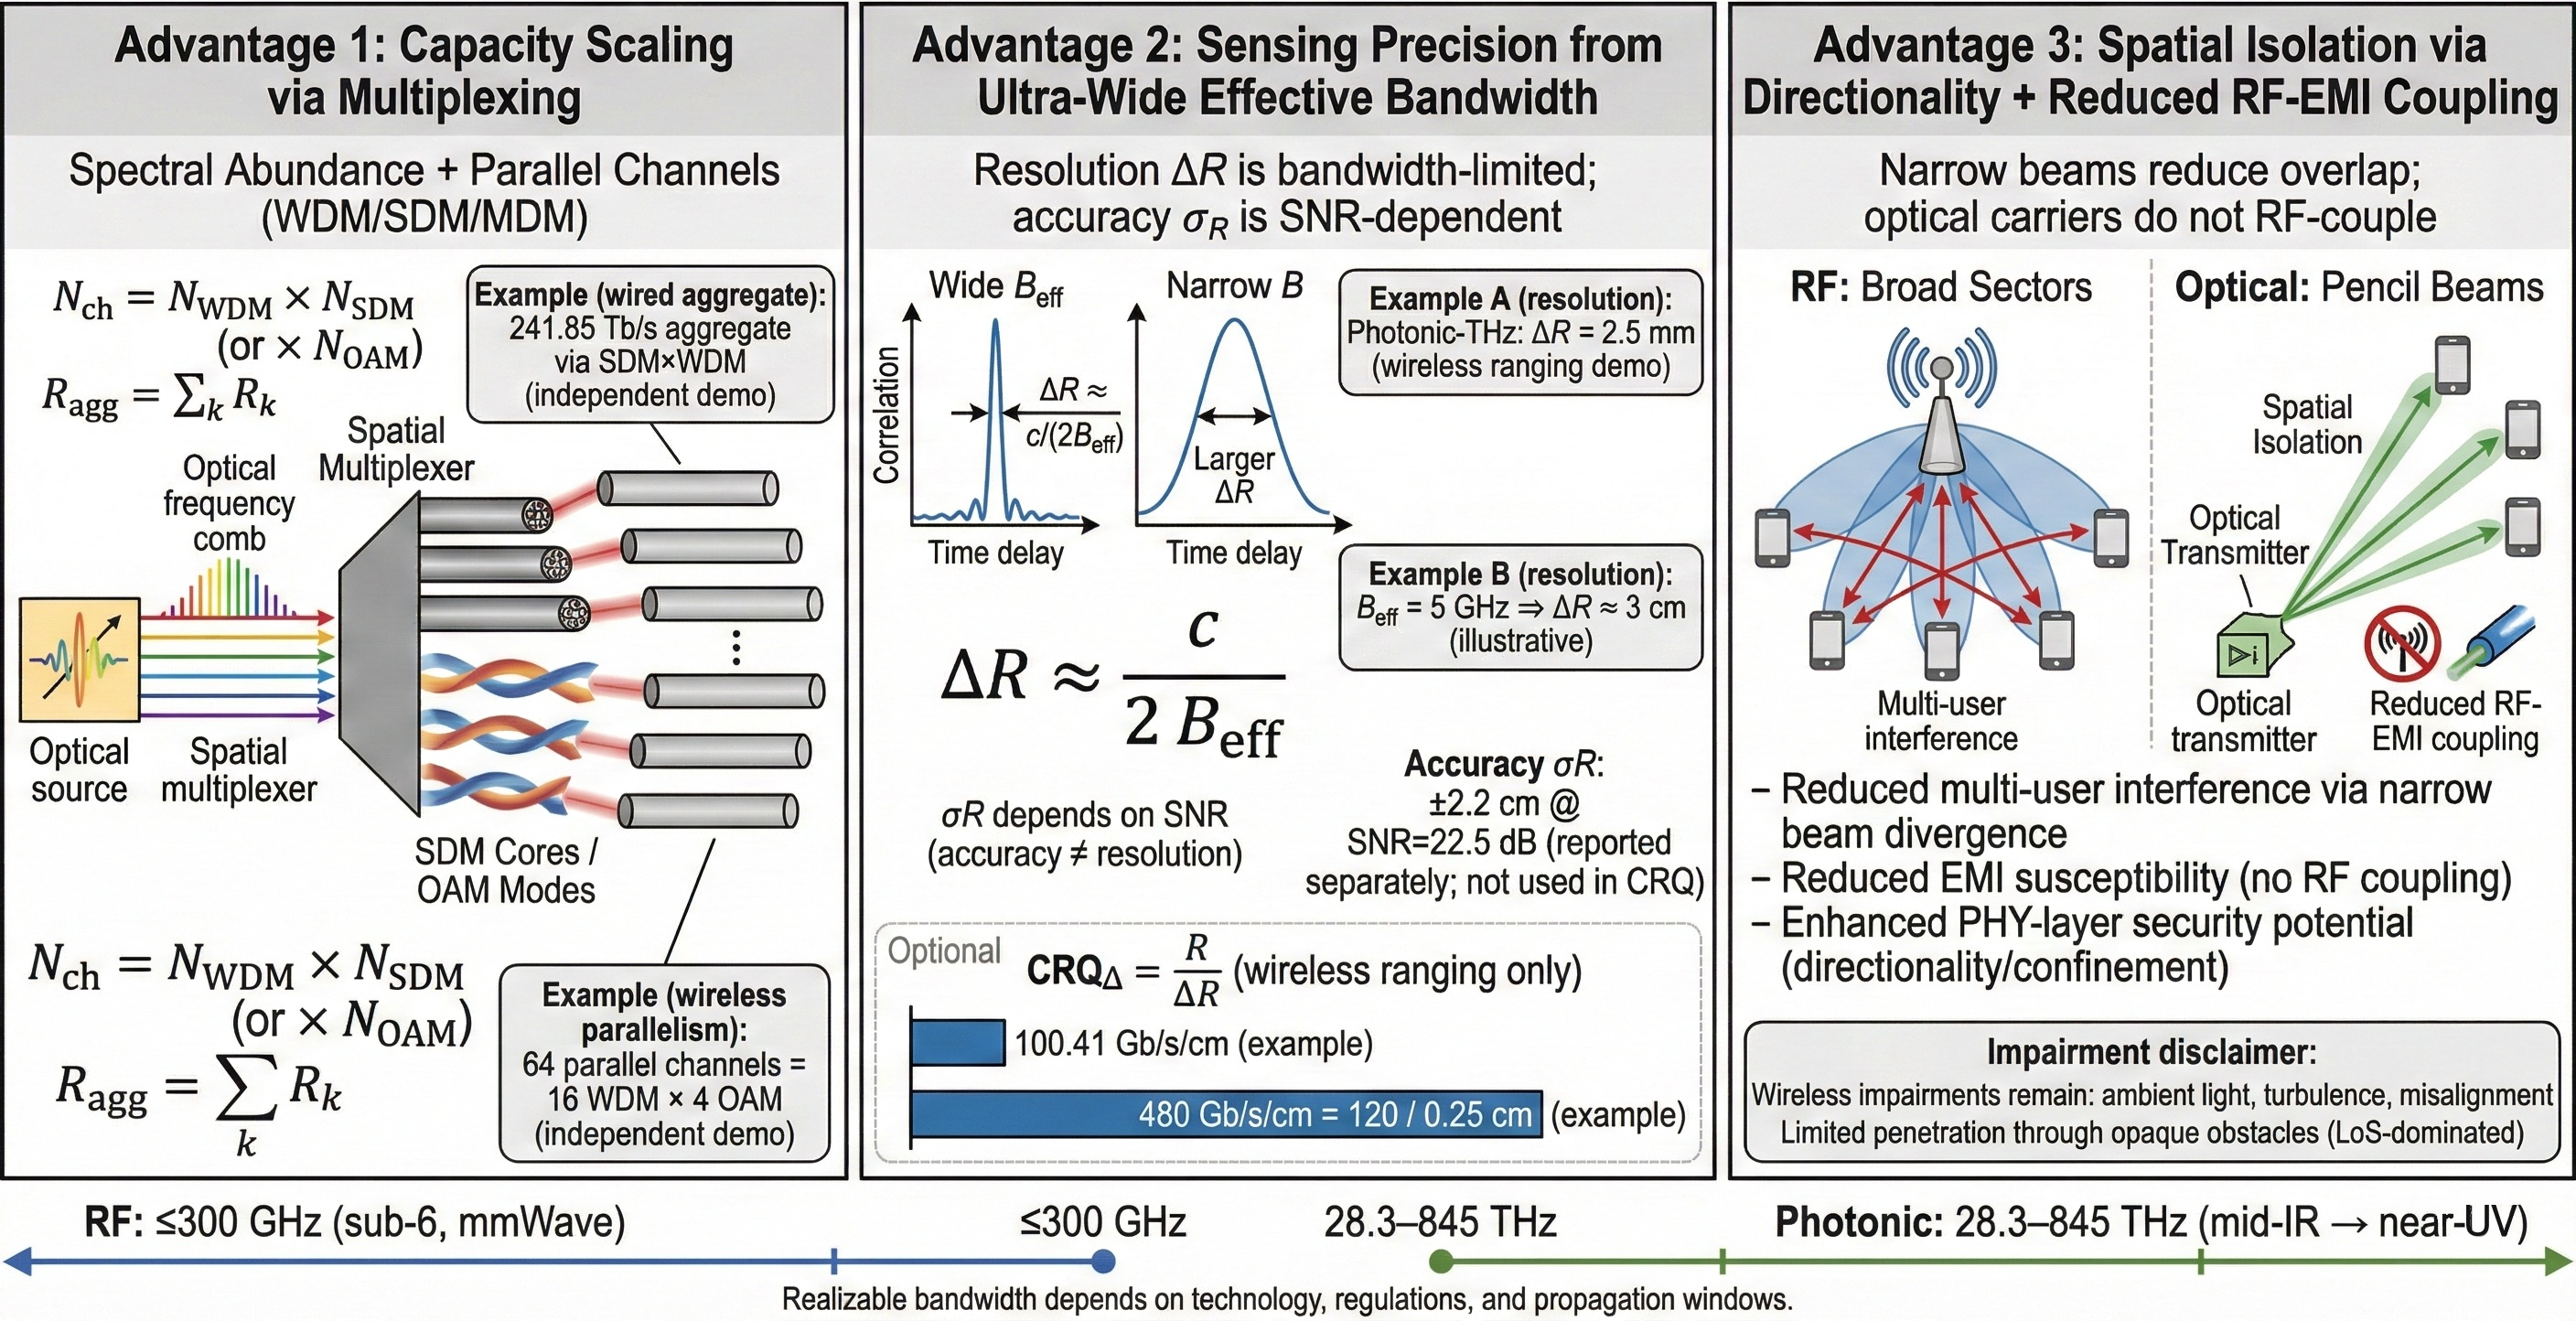
\includegraphics[width=\linewidth]{figures/fig2.jpg}
    \caption{Physical basis of the three optical advantages: dense multiplexing for capacity scaling, ultra-wide effective bandwidth for fine ranging and high $\text{CRQ}_{\Delta}$, and narrow beams for spatial isolation with lower RF-EMI coupling.}
    \label{fig:fig2}
\end{figure*}

% ---- Moved block: fig:fig3 ----
\begin{figure*}[!t]
    \centering
    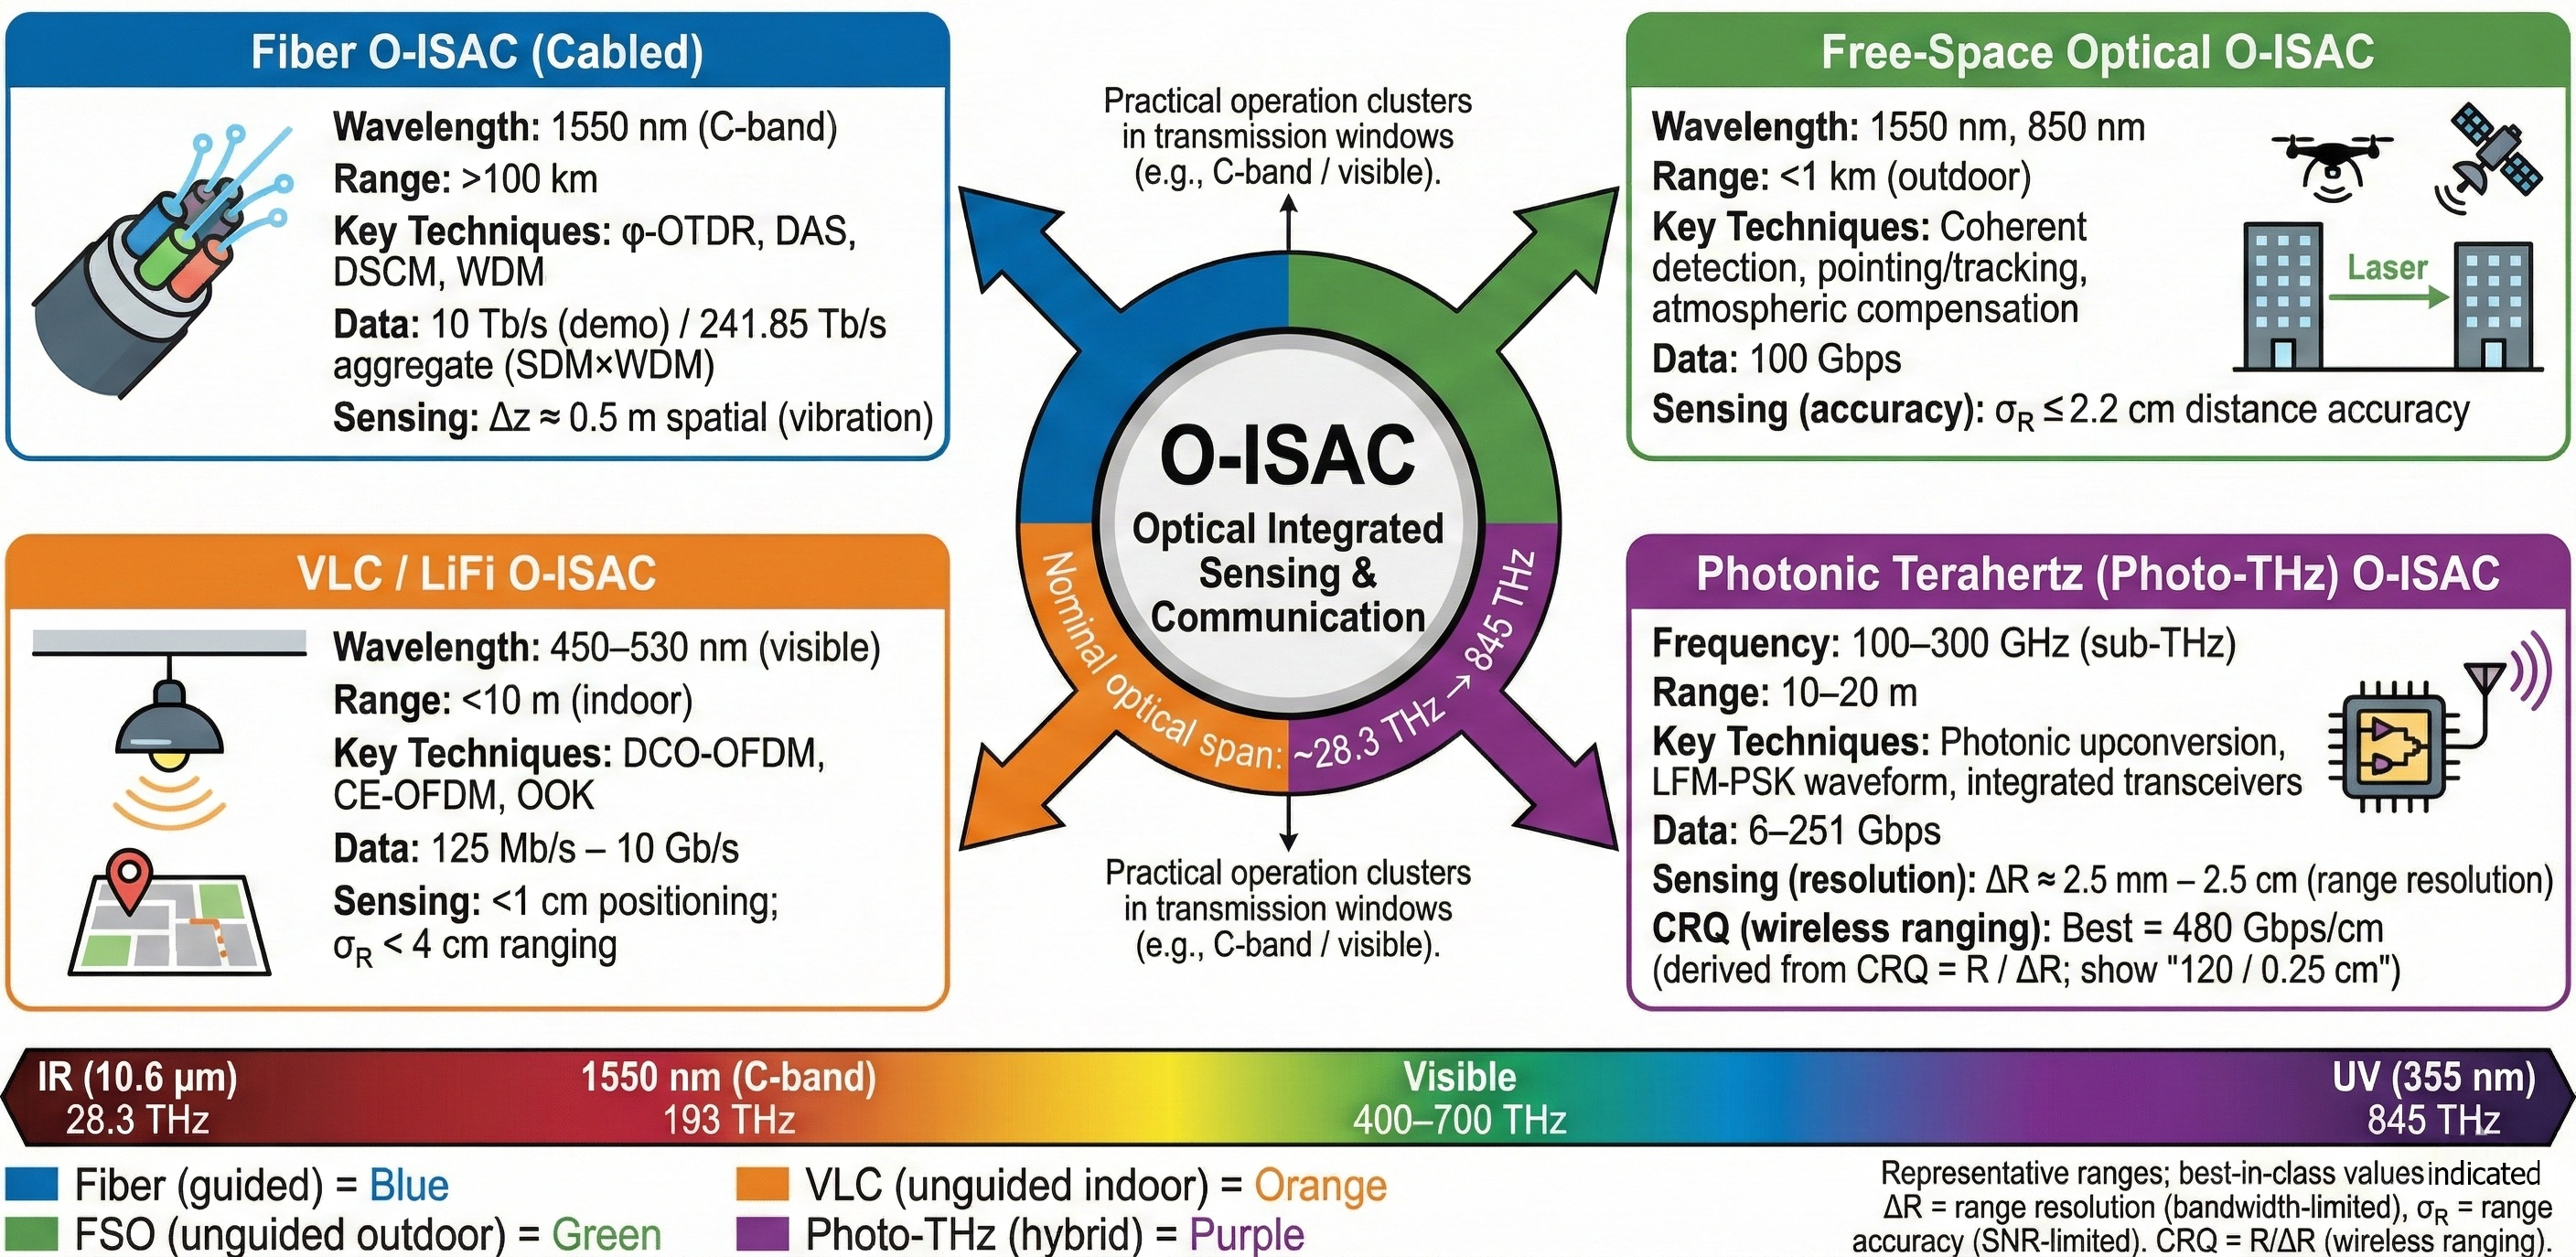
\includegraphics[width=\linewidth]{figures/fig3.jpg}
    \caption{Preview of the four modality families in the 220-study PRISMA corpus: fiber, FSO, VLC/LiFi, and photonic-THz, distinguished by operating window, dominant impairment, and representative sensing--communication tasks.}
    \label{fig:fig3}
\end{figure*}

% ---- Moved block: fig:fig_ii_2 ----
\begin{figure*}[!t]
    \centering
    
\includegraphics[width=\linewidth]{figures/fig_ii_2.jpg}
    \caption{Metric contract and admissible comparison map for O-ISAC. The figure links effective bandwidth to \(\Delta r_{\min}\), delay/time-of-flight to range, and matched \(R\) plus \(\Delta r_{\min}\) to \(\mathrm{CRQ}_{\Delta}\), while keeping \(\sigma_r\), CRB/FIM, \(\Delta z\), and OSNR versus SNR/ESNR explicitly separated. Green links are admissible, dashed gray links are contextual, and red links are forbidden substitutions without an explicit receiver/noise model.}
    \label{fig:fig_ii_2}
\end{figure*}

% ---- Moved block: fig:fig_iv_2 ----
\begin{figure*}[!t]
    \centering
    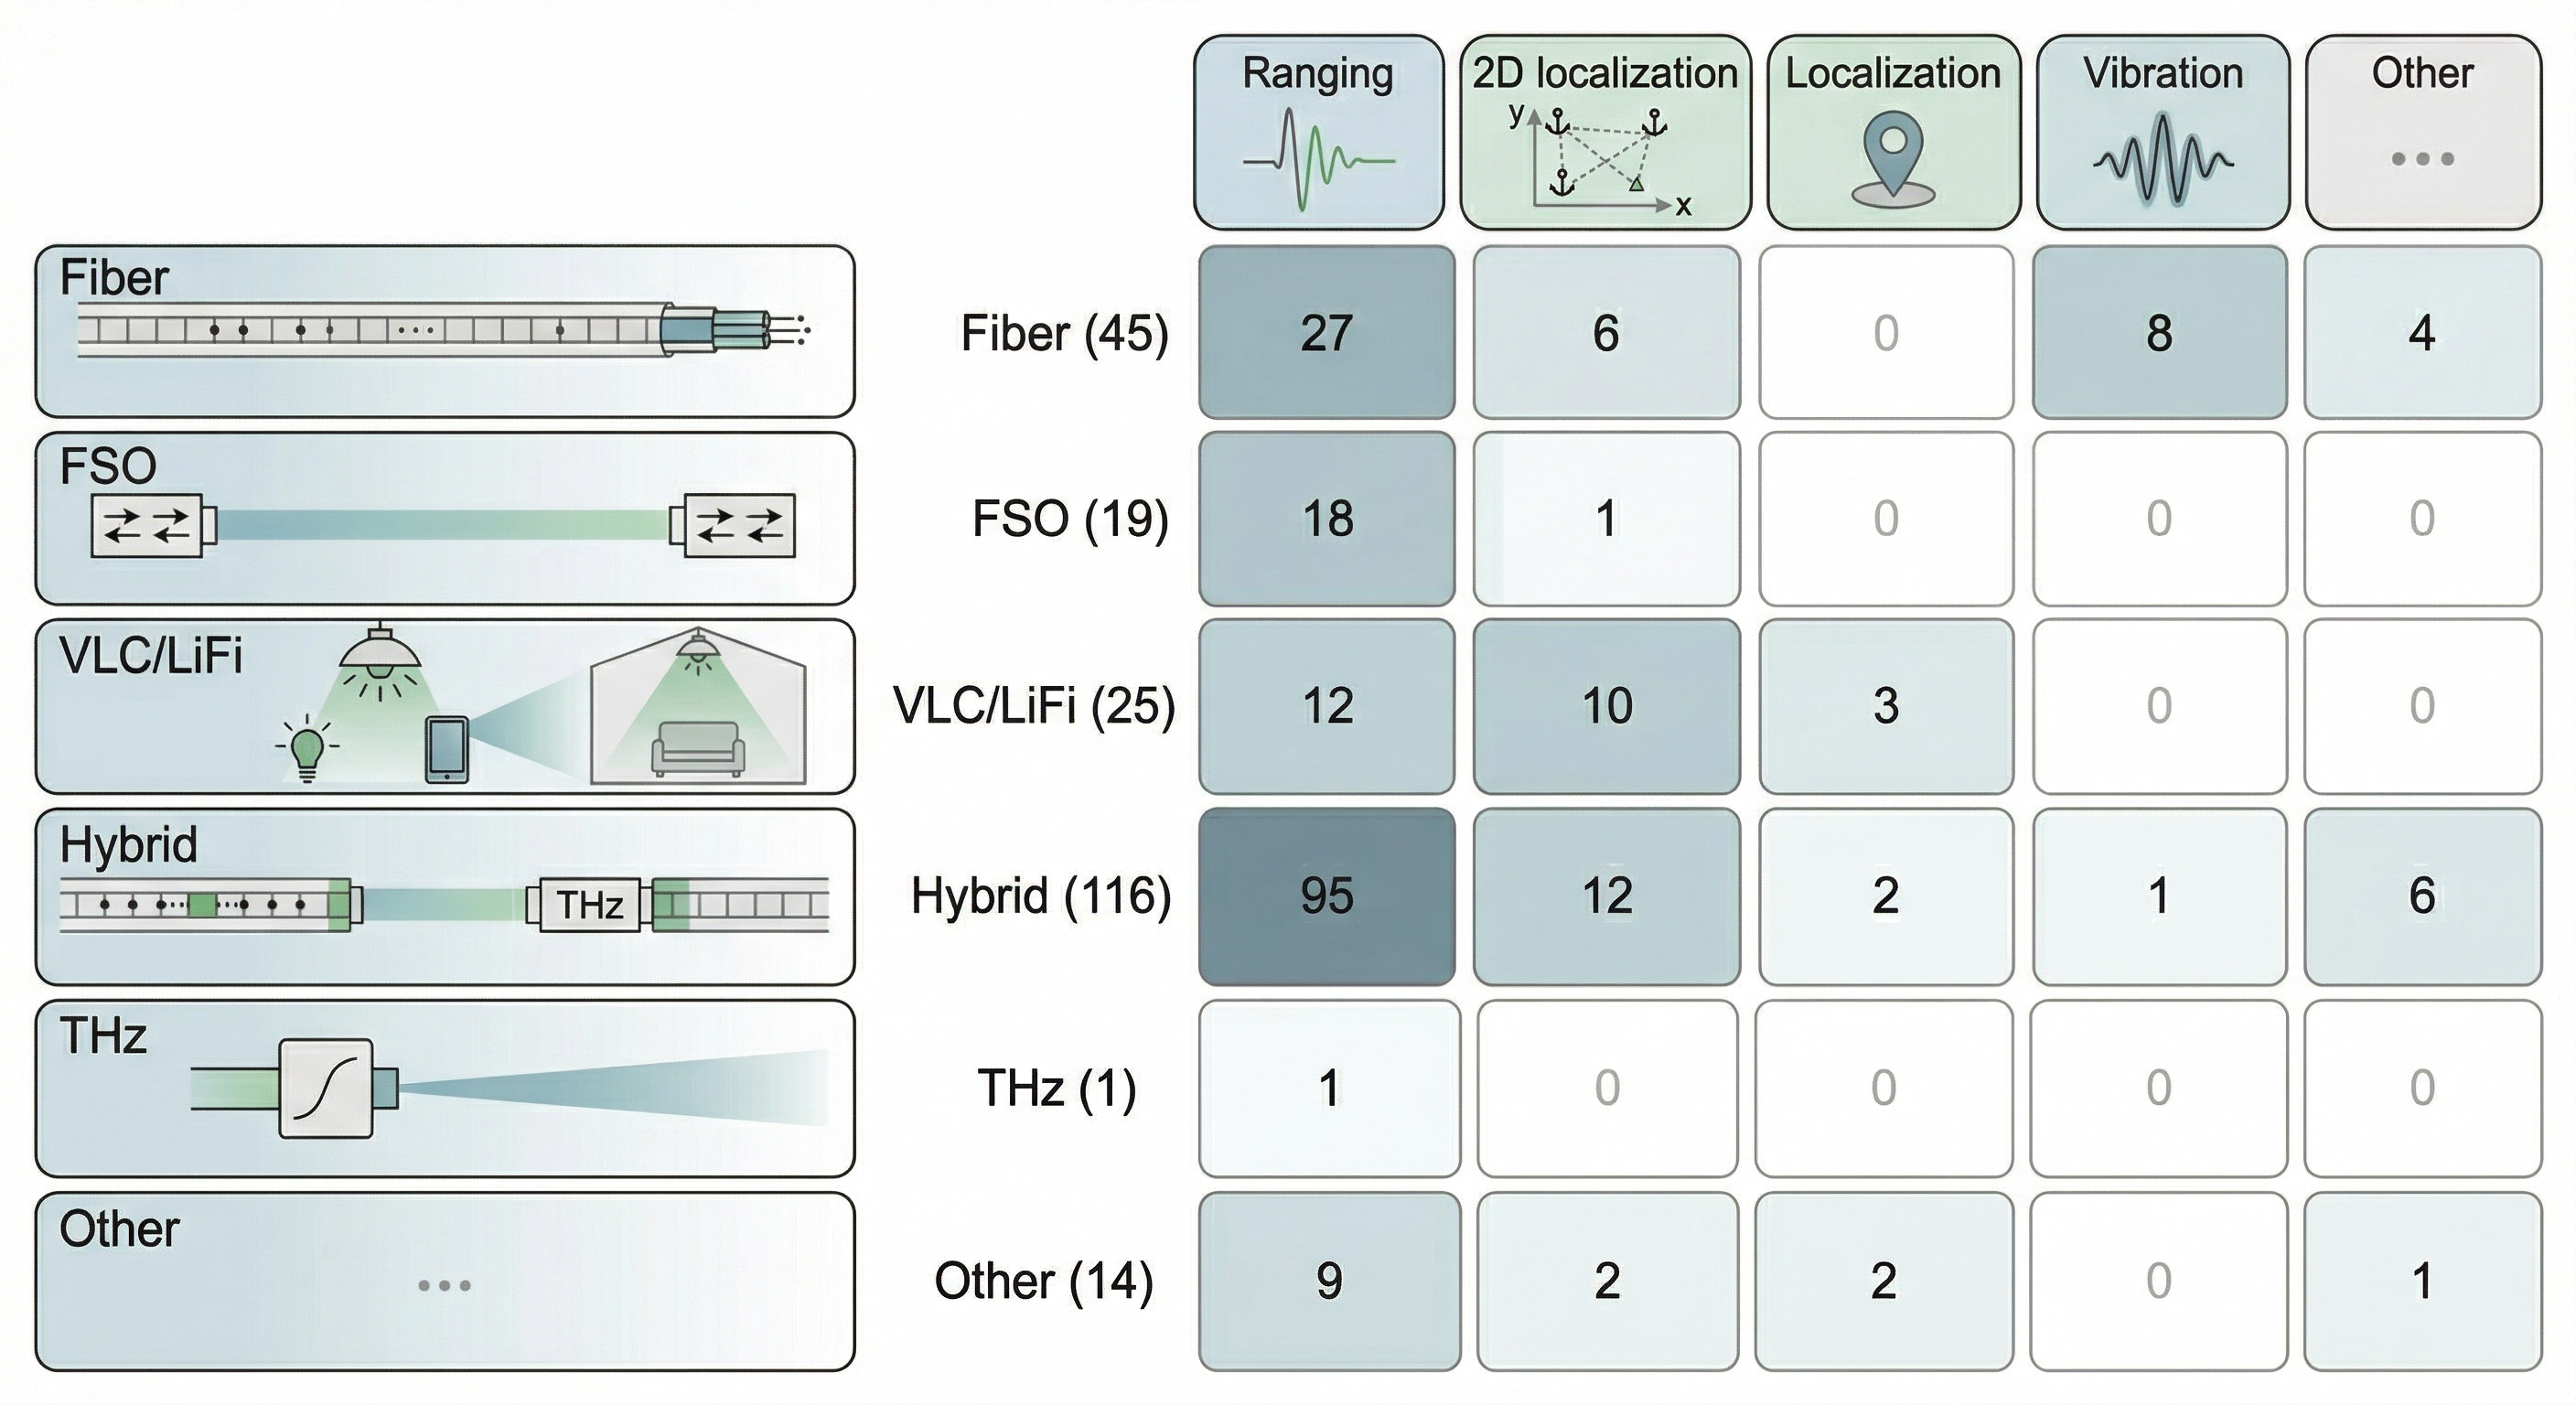
\includegraphics[width=\linewidth]{figures/fig_iv_2.jpg}
    \caption{Reader-facing medium-task specialization view for O-ISAC. The figure highlights how dominant medium classes connect to representative sensing emphases, including ranging, VLC/LiFi localization, fiber vibration monitoring, and hybrid multi-task breadth, without implying that prevalence means superiority. It complements the denser cluster-level synthesis in Table~\ref{tab:taxonomy_clusters}.}
    \label{fig:fig_iv_2}
\end{figure*}

% ---- Moved block: fig:fig_v_2 ----
\begin{figure*}[!t]
    \centering
    
\includegraphics[width=\linewidth]{figures/fig_v_2.png}
    \caption{Reader-facing sparse frontier for the CRQ-valid subset of Section V. Faint markers denote the 20 governance-usable points and outlined markers the 2 nondominated Pareto points. The figure is therefore a bounded frontier illustration rather than a full-cloud or modality-ranking view.}
    \label{fig:fig_v_2}
\end{figure*}

% ---- Moved block: fig:fig_vi_1 ----
\begin{figure*}[!t]
    \centering
    
\includegraphics[width=\linewidth]{figures/fig_vi_1.jpg}
    \caption{Section VI enabler landscape across medium classes. OPA and ORIS are the primary programmable-enabler evidence cores, whereas PIC, photonic generation, and programmable photonics remain supporting substrate families; medium-wise concentrations are shown without turning contextual traces into maturity claims.}
    \label{fig:fig_vi_1}
\end{figure*}

% ---- Moved block: fig:fig_vii_1 ----
\begin{figure*}[!t]
    \centering
    
\includegraphics[width=\linewidth]{figures/fig_vii_1.jpg}
    \caption{Cross-domain deployment synthesis of O-ISAC applications over the 220-paper corpus and 48 micro-domains. The five macro-domain panels summarize recurring deployment motifs and compact communication-/sensing-plane cues; OPA/ORIS mentions remain contextual.}
    \label{fig:fig_vii_1}
\end{figure*}

% ---- Moved block: eq:nlse_conceptual ----
\begin{equation}
    \begin{split}
        \frac{\partial A(z,t)}{\partial z}
         & =
        -\frac{\alpha}{2}A
        -j\frac{\beta_2}{2}\frac{\partial^2 A}{\partial t^2} \\
         & \quad
        +j\gamma |A|^2 A
        +\eta(z,t)
    \end{split}
    \label{eq:nlse_conceptual}
\end{equation}

% ---- Moved line-range block: Section VI resource-optimization equations, original lines 1675-1686 ----
\begin{equation}
    \begin{split}
        \mathcal U=\{x(t):x(t)\ge 0,\;\mathbb{E}[x(t)]\le \bar P, \\
        \qquad \max_t x(t)\le P_{\max}\}
    \end{split}
\end{equation}
\begin{equation}
    \begin{split}
        \max_{\mathbf{w},\Theta,\,x\in\mathcal U}\; & \alpha R(\mathbf{w},\Theta)                                       \\
                                                    & -(1-\alpha)\,\mathrm{CRB}(\mathbf{w},\Theta),\quad \alpha\in[0,1]
    \end{split}
\end{equation}

% ---- Moved line-range block: Section VI multi-user/security equations, original lines 1766-1799 ----
\begin{equation}
    \begin{split}
        \max_{\{\mathbf{w}_k\},\Theta}\; & \sum_{k}\omega_k\log\!\left(1+\mathrm{SINR}_k\right) \\
                                         & -\lambda\,\mathrm{CRB}(\Theta)
    \end{split}
\end{equation}
\begin{equation}
    \begin{split}
        \text{s.t.}\quad & \sum_k\|\mathbf{w}_k\|_2^2\le P, \\
                         & \theta_n\in\mathcal Q.
    \end{split}
\end{equation}

This formulation makes communication, sensing, and ORIS quantization constraints explicit in one multi-user program \cite{O_ISAC_061,O_ISAC_091,O_ISAC_127}. Its interpretation still requires fixed detection semantics for $\mathrm{SINR}_k$ and a role-consistent sensing objective rather than a mixed resolution-accuracy score. At this point, the narrative starts to connect directly to Section VII: once user count, fusion policy, fairness, and control overhead dominate, the key question is whether a deployment setting can absorb the coordination cost.

\textbf{VI-E takeaway.} Multi-user optical O-ISAC is supported by a growing set of targeted studies, but network-level overhead metrics, control-plane timing, and cooperative benchmark contracts remain under-standardized. This is where enabler analysis becomes deployment analysis: coordination cost, fairness, and sensing-fusion policy begin to determine application readiness, which in turn motivates VI-F.

\subsection{AI/ML and Security-Aware Adaptation}

AI-assisted adaptation and security-aware design are emerging layers in O-ISAC, especially in dynamic channels where static policies may underperform. At the study-level tag view fixed in Section I, machine learning appears in 53 studies, but only a narrower subset supports direct interpretation as reproducible adaptation or security-aware control in Section VI. The available literature therefore contains targeted reports of learning-driven adaptation, learning-assisted compensation and receiver refinement, and learning-based angle estimation, together with secrecy, authentication, and resilience formulations, but jointly validated AI-plus-security optical benchmarks remain limited \cite{O_ISAC_017,O_ISAC_127,O_ISAC_145,O_ISAC_156,O_ISAC_157,O_ISAC_163,O_ISAC_245}. In the review flow, this subsection functions as a forward-looking systems layer rather than a co-equal replacement for the physical enabler evidence in VI-A.

A compact secrecy and robust-control anchor is
\begin{equation}
    R_s=[R_b-R_e]^+,
\end{equation}
\begin{equation}
    \begin{split}
        \max_{\mathbf{u}}\;\min_{a\in\mathcal A}\; & \alpha R(\mathbf{u})+\beta R_s(\mathbf{u},a) \\
                                                   & -(1-\alpha-\beta)\,\mathrm{CRB}(\mathbf{u}),
    \end{split}
\end{equation}
\begin{equation}
    \alpha\ge 0,\;\beta\ge 0,\;\alpha+\beta\le 1,
\end{equation}

% ---- Moved line-range block: Section VII organizational application equations, original lines 1928-2051 ----
\begin{equation}
    \begin{split}
        \max_{u,\pi,T}\  & \alpha R_{\mathrm{comm}}(u,\pi;s)      \\
                         & - (1-\alpha) J_{\mathrm{sense}}(u,T;s)
    \end{split}
\end{equation}
\begin{equation}
    \begin{split}
        \text{s.t.}\  & \sum_{k=1}^{K} p_k \le P_{\mathrm{avg}}, \\
                      & 0 \le p_k \le P_m,\ \forall k,
    \end{split}
\end{equation}
\begin{equation}
    \mathrm{BER}(u,\pi;s) \le \beta_{\mathrm{rel}}.
\end{equation}

Here, $u$ collects waveform/link-adaptation settings and $s$ the deployment state; $R_{\mathrm{comm}}$ and BER capture the communication plane, while $J_{\mathrm{sense}}$ acts as a ranging-error surrogate \cite{O_ISAC_034,O_ISAC_048}. The cap $P_m$ follows reported subcarrier-power limits, and the BER bound is an illustrative service target rather than a universal threshold \cite{O_ISAC_034,O_ISAC_048}.

\textbf{Key takeaway.} VII-A shows that fiber corridors and monitored access links can jointly sustain sensing readout and high-rate communication, but the evidence remains scenario dependent and keeps BER and ranging-error families separate.

\subsection{Indoor Environments}

VII-B uses shared lighting-centric infrastructure to deliver service while sensing user or room state in the same transceiver workflow. The evidence spans retroreflective VLC localization, gesture-aware lamps, distributed O-AP deployments, and multi-user VLC-CDMA, with reported outcomes ranging from BER-tracked links plus positioning RMSE to gesture recognition above 90\% at 220 kbps and coordinate MSE below $10^{-4}$ in two-phase LED O-ISAC \cite{O_ISAC_011,O_ISAC_030,O_ISAC_108,O_ISAC_388}.

\textbf{Math anchor.}
\begin{equation}
    \begin{split}
        \min_{u}\  & \alpha\,\mathrm{BER}(u;s) + (1-\alpha)\,\mathrm{MSE}_{\mathrm{pos}}(u;s), \\
                   & s=(g_{\mathrm{room}},\rho_{\mathrm{user}}).
    \end{split}
\end{equation}

Here, $u$ denotes indoor control variables over the shared communication-sensing stack; BER represents communication quality and position-coordinate MSE the sensing plane \cite{O_ISAC_108,O_ISAC_388}.

\textbf{Key takeaway.} Indoor evidence couples practical service with localization or gesture sensing on shared optical infrastructure; the clearest dual-plane reporting comes from retroreflective and distributed O-AP cases, while optical-tag and intelligent-terminal VLC extensions remain more communication- or access-oriented than sensing-rich \cite{O_ISAC_291,O_ISAC_386}.

\subsection{Automotive Transportation}

VII-C covers moving-road deployments that require optical connectivity and environment-aware operation in the same workflow, including taillight/headlight signaling, OCC reception, and vehicular FSO relays. Representative cases include autonomous-vehicle ISAC-OW with a 100.011 m LiDAR estimate for a 100 m target and BER-versus-SNR reporting, OCC-based V2X with normalized sensing and communication gains under mobility, LiDAR-aided simulation pipelines for vehicular wireless-link evaluation, and vehicular VLC/FSO links reporting received-power-ratio, delay-spread, or ToF-oriented CRB/RMSE together with BER or achievable rate \cite{O_ISAC_003,O_ISAC_055,O_ISAC_060,O_ISAC_109,O_ISAC_164}.

\textbf{Math anchor.}
\begin{equation}
    \begin{split}
        \max_{u,\pi,T}\  & \alpha R_{\mathrm{comm}}(u,\pi;s)    \\
                         & -(1-\alpha)J_{\mathrm{sense}}(u,T;s)
    \end{split}
\end{equation}
\begin{equation}
    \begin{split}
        \text{s.t.}\  & \sum_{k=1}^{K} p_k \le P_{\mathrm{avg}},       \\
                      & 0 \le p_k \le P_m,\ \forall k,                 \\
                      & \mathrm{BER}(u,\pi;s)\le \beta_{\mathrm{rel}}.
    \end{split}
\end{equation}

The sensing plane is represented by LiDAR ranging, gain, or CRB/RMSE descriptors, while the communication plane is represented by BER or achievable rate.

\textbf{Key takeaway.} Vehicular optical ISAC is highly condition dependent, but the cited studies consistently keep sensing-plane and comm-plane metrics separate. All current cases remain Conventional because the deployments are built around optical sources, receivers, and DSP rather than explicit ORIS/OPA control.

\subsection{Underwater and Harsh-Environment OWC}

VII-D emphasizes operation under attenuation, turbulence, and environmental variability, mainly through secure underwater links and subsea cable monitoring. Representative studies pair BER reduction and secrecy-rate outcomes with environmental-state MAE of 0.008 PSU, combine 20 GBaud DP-QAM16 transmission and Q-factor gains with in-line temperature sensing at $0.0625\,^{\circ}\mathrm{C}$ resolution, and extend the vertical toward deep-ocean salinity or bio-environment monitoring through integrated optical sensing-communication platforms \cite{O_ISAC_027,O_ISAC_127,O_ISAC_130,O_ISAC_220}.

\textbf{Math anchor.}
\begin{equation}
    \begin{split}
        \max_u\  & \alpha R_{\mathrm{comm}}(u;s)      \\
                 & -(1-\alpha)J_{\mathrm{sense}}(u;s)
    \end{split}
\end{equation}
\begin{equation}
    \begin{split}
        \text{s.t.}\  & \mathrm{BER}(u;s)\le \epsilon_{\mathrm{comm}},  \\
                      & \mathrm{MAE}(u;s)\le \epsilon_{\mathrm{sense}}.
    \end{split}
\end{equation}

\textbf{Key takeaway.} This vertical is governed more by environmental stress and secure operation than by headline rate alone; sensing is typically environmental-state or thermal monitoring, while communication remains BER- and secrecy-oriented.

\subsection{Space and Satellite Networks}

VII-E covers satellite-network settings where optical inter-satellite connectivity and relay behavior share payload chains with remote-observation or environment-aware sensing. The evidence spans ISL backbone transport, Doppler-robust LEO payloads with range resolution better than 0.146 m plus 29.99 Mbps and BER below the 7\% pre-FEC threshold, adaptive satellite-ground laser links, SLR-style ranging/data transfer integration, and multi-beam payloads with 2.4 Gbps communication plus BER/EVM and remote-sensing descriptors \cite{O_ISAC_089,O_ISAC_137,O_ISAC_187,O_ISAC_195,O_ISAC_252}.

\textbf{Math anchor.}
\begin{equation}
    \begin{split}
        \max_{u\in\mathcal{U}(s)}\; & \alpha R_{\mathrm{comm}}(u;s)      \\
                                    & -(1-\alpha)J_{\mathrm{sense}}(u;s)
    \end{split}
\end{equation}
\begin{equation}
    \begin{split}
        \text{s.t. } & \mathrm{BER}(u;s)\le\epsilon_{\mathrm{comm}},           \\
                     & \rho_{\mathrm{range}}(u;s)\le\epsilon_{\mathrm{sense}}, \\
                     & s=(s_{\mathrm{LEO}},s_{\mathrm{mb}}).
    \end{split}
\end{equation}

\textbf{Key takeaway.} Space-satellite O-ISAC spans ISL transport, Doppler-robust payloads, SLR integration, and multi-beam observation payloads. Communication and sensing are both explicit but remain different metric families, and all scenarios still read as Conventional because no source establishes OPA- or ORIS-dominant control.

\subsection{Cross-Domain Application Synthesis}

VII-F is a cross-domain synthesis layer rather than a single vertical. Under the frozen-manuscript policy, Section VII uses strict evidence counts over the canonical 220-paper corpus and 48 micro-domains as its primary view, with strongest coverage in smart infrastructure, automotive transportation, and indoor environments; structured \texttt{study\_flag\_count} values are kept only in VII-G as a secondary audit lens. Representative transfer motifs include 10.4 km coherent fiber carriage with 1 m sensing resolution, Doppler-robust LEO payload links, vehicular OC-ISAC camera systems with normalized sensing/communication gains, and indoor localization-plus-access deployments with distributed O-APs \cite{O_ISAC_011,O_ISAC_074,O_ISAC_108,O_ISAC_164,O_ISAC_187}.

\textbf{Math anchor.}
\begin{equation}
    \begin{split}
        \max_{x,z,g,y}\; & \sum_{d \in D} W_d z_d + \sum_{a \in A} V_a g_a \\
                         & - \lambda \sum_{d<q} L_{d,q}(1-y_{d,q}).
    \end{split}
\end{equation}
\begin{equation}
    \begin{split}
        \text{s.t. } & z_d \le \sum_{i=1}^{N} M_{i,d}x_i, \\
                     & g_a \le \sum_{i=1}^{N} U_{i,a}x_i, \\
                     & \sum_{i=1}^{N}x_i \le B.
    \end{split}
\end{equation}
\begin{equation}
    \begin{split}
        y_{d,q}\le z_d,\quad  & y_{d,q}\le z_q,            \\
        x_i \in \{0,1\},\quad & z_d,g_a,y_{d,q}\in\{0,1\}.
    \end{split}
\end{equation}

% ---- Moved line-range block: Section VIII roadmap utility equation, original lines 2156-2169 ----
\begin{equation}
    \begin{aligned}
        u             & = (u_{\mathrm{profile}},u_{\mathrm{placement}},u_{\mathrm{dsp}}), \\
        \max_{u}\quad & J_{\mathrm{perf}}(u),                                             \\
        \text{s.t.}\quad
                      & u_{\mathrm{profile}} \in \mathcal{U}_{\mathrm{SMART\_conform}},   \\
                      & (u_{\mathrm{placement}},u_{\mathrm{profile}})                     \\
                      & \qquad \in \mathcal{U}_{\mathrm{blank\_allocation}},              \\
                      & (u_{\mathrm{dsp}},u_{\mathrm{placement}})                         \\
                      & \qquad \in \mathcal{U}_{\mathrm{dsp\_compatible}},                \\
                      & u \in \mathcal{U}_{\mathrm{PtMP\_attribution}},                   \\
                      & J_{\mathrm{perf}}(u) \in \mathcal{J}_{\mathrm{QoS\_acceptable}}.
    \end{aligned}
\end{equation}

% ---- Moved line-range block: Section VIII hardware roadmap equation, original lines 2196-2206 ----
\begin{equation}
    \begin{aligned}
        u                 & = (u_{arch},u_{proc},u_{ctrl}),                             \\
        \max_{u} \quad    & U_{perf}(u;s)                                               \\
                          & = \beta_c U_{comm}(u;s_{comm})+\beta_s U_{sens}(u;s_{sens}) \\
        \text{s.t.} \quad & C_{hw}(u;s) \le C_{max},                                    \\
                          & L_{hw}(u;s) \le L_{max},                                    \\
                          & P_{hw}(u;s) \le P_{max},                                    \\
                          & O_{ctrl}(u;s) \le O_{max}.
    \end{aligned}
\end{equation}

% ---- Moved line-range block: Section VIII channel/security roadmap equations, original lines 2233-2242 ----
\begin{equation}
    \max_{\pi}\; U_{\mathrm{eval}}(\pi).
\end{equation}
\begin{equation}
    \begin{split}
        \text{s.t.}\;               & \pi \in \Pi_{\mathrm{contract}},                   \\
        \Pi_{\mathrm{contract}} =\; & \{\kappa_{\mathrm{cond}},\,\gamma_{\mathrm{geom}}, \\
                                    & \mu_{\mathrm{metric}},\,\delta_{\mathrm{prov}}\}
    \end{split}
\end{equation}

% ---- Moved line-range block: Section VIII deployment roadmap equation, original lines 2269-2277 ----
\begin{equation}
    \begin{aligned}
        u                 & = (u_{\mathrm{auth}},u_{\mathrm{mon}},u_{\mathrm{priv}}), \\
        \max_{u} \quad    & U_{\mathrm{service}}(u)                                   \\
        \text{s.t.} \quad & R_{\mathrm{int}}(u) \le \varepsilon_{\mathrm{int}},       \\
                          & L_{\mathrm{priv}}(u) \le \varepsilon_{\mathrm{priv}},     \\
                          & A_{\mathrm{auth}}(u) \ge \tau_{\mathrm{auth}}.
    \end{aligned}
\end{equation}

% ---- Moved line-range block: Section VIII dependency synthesis equation, original lines 2304-2316 ----
\begin{equation}
    \begin{aligned}
        u                 & = (u_{\mathrm{arch}},u_{\mathrm{api}},u_{\mathrm{stack}},       \\
                          & \qquad u_{\mathrm{model}},u_{\mathrm{audit}}),                  \\
        \max_{u} \quad    & U_{\mathrm{deploy}}(u)                                          \\
        \text{s.t.} \quad & g_{\mathrm{ready}}(u) \ge 0,                                    \\
                          & \operatorname{compat}_{\mathrm{infra}}(u)=1,                    \\
                          & \operatorname{budget}_{\mathrm{edge}}(u) \le B_{\mathrm{edge}}, \\
                          & \operatorname{budget}_{\mathrm{bw}}(u) \le B_{\mathrm{bw}},     \\
                          & \operatorname{valid}_{\mathrm{model}}(u)=1,                     \\
                          & \operatorname{prov}_{\mathrm{audit}}(u)=1.
    \end{aligned}
\end{equation}

% ---- Moved line-range block: Section VIII audit-consistency equation, original lines 2452-2459 ----
\begin{equation}
    \begin{aligned}
        \max_{x \in \{0,1\}^N}\quad & \sum_{i=1}^{N} w_i x_i                                                     \\
        \text{s.t.}\quad            & \sum_{i=1}^{N} c_i x_i \le B,                                              \\
                                    & \mathrm{cover}_d(x) \ge z_d,\quad d \in \{A,B,C,D,E\}_{\mathrm{selected}}, \\
                                    & \mathrm{risk\_flag}(x) \le R_{\max}.
    \end{aligned}
\end{equation}
